\documentclass{standalone}
\usepackage{tikz}
\usetikzlibrary{patterns, positioning}

\begin{document}
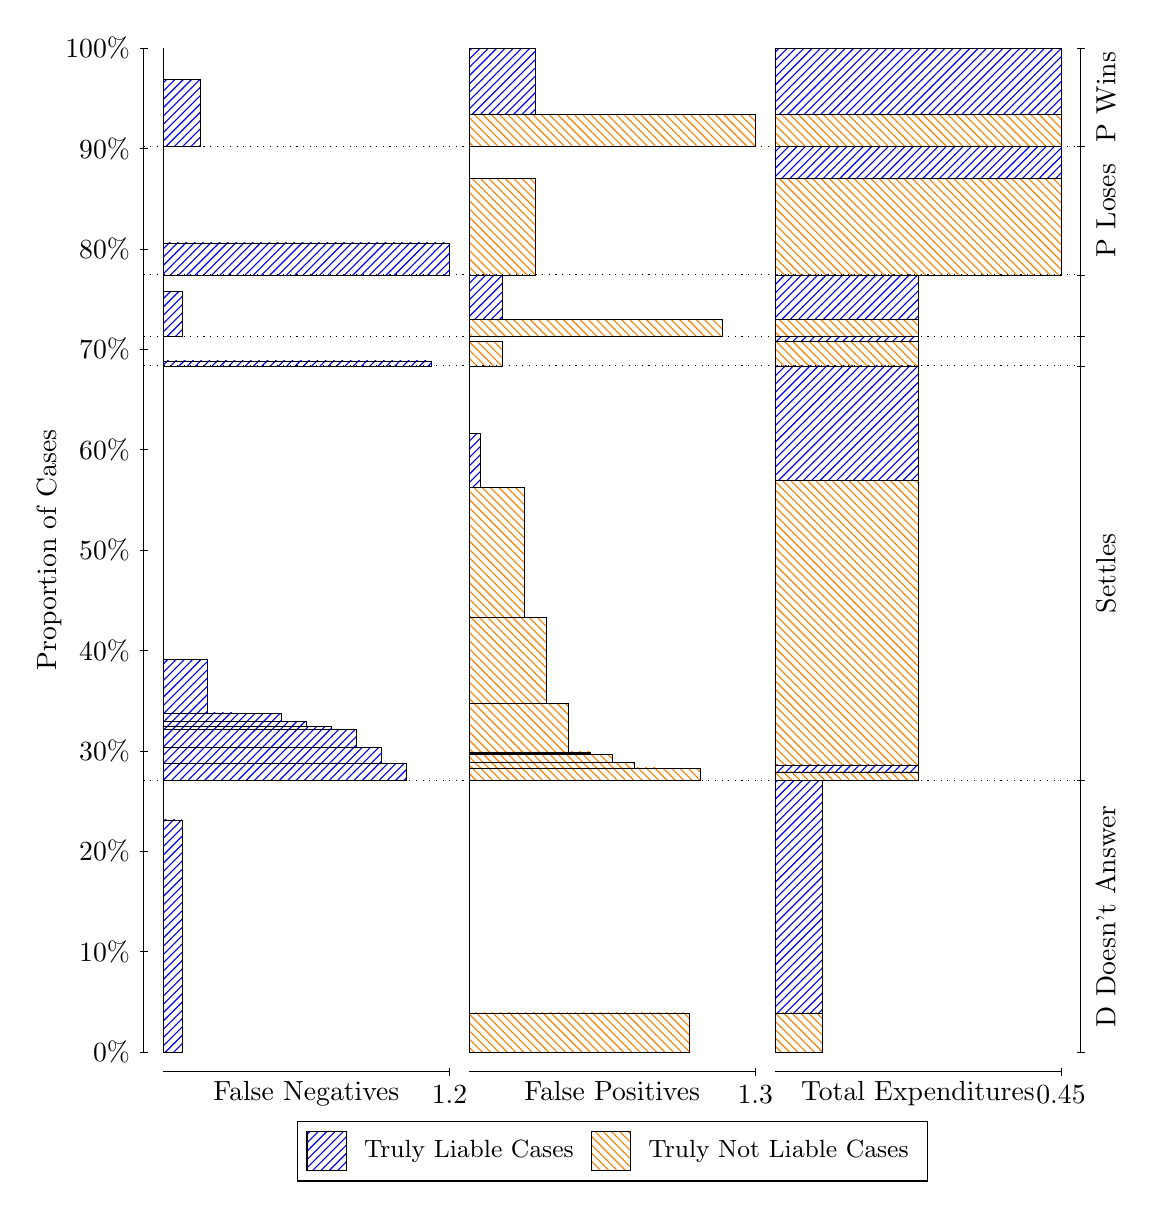
\begin{tikzpicture}
\draw[black, very thin] (1.5,1.75) -- (1.5,14.5);
\node[rotate=90, anchor=center] at (0.3, 8.125) {Proportion of Cases};
\draw[black, very thin] (1.45,1.75) -- (1.55,1.75);
\node[anchor=east] at (1.45, 1.75) {0\%};
\draw[black, very thin] (1.45,3.025) -- (1.55,3.025);
\node[anchor=east] at (1.45, 3.025) {10\%};
\draw[black, very thin] (1.45,4.3) -- (1.55,4.3);
\node[anchor=east] at (1.45, 4.3) {20\%};
\draw[black, very thin] (1.45,5.575) -- (1.55,5.575);
\node[anchor=east] at (1.45, 5.575) {30\%};
\draw[black, very thin] (1.45,6.85) -- (1.55,6.85);
\node[anchor=east] at (1.45, 6.85) {40\%};
\draw[black, very thin] (1.45,8.125) -- (1.55,8.125);
\node[anchor=east] at (1.45, 8.125) {50\%};
\draw[black, very thin] (1.45,9.4) -- (1.55,9.4);
\node[anchor=east] at (1.45, 9.4) {60\%};
\draw[black, very thin] (1.45,10.675) -- (1.55,10.675);
\node[anchor=east] at (1.45, 10.675) {70\%};
\draw[black, very thin] (1.45,11.95) -- (1.55,11.95);
\node[anchor=east] at (1.45, 11.95) {80\%};
\draw[black, very thin] (1.45,13.225) -- (1.55,13.225);
\node[anchor=east] at (1.45, 13.225) {90\%};
\draw[black, very thin] (1.45,14.5) -- (1.55,14.5);
\node[anchor=east] at (1.45, 14.5) {100\%};

\draw[black, very thin] (13.4,1.75) -- (13.4,14.5);
\draw[black, very thin] (13.35,1.75) -- (13.45,1.75);
\node[anchor=west] at (13.35, 1.75) {};
\draw[black, very thin] (13.35,5.1953) -- (13.45,5.1953);
\node[anchor=west] at (13.35, 5.1953) {};
\draw[black, very thin] (13.35,10.464) -- (13.45,10.464);
\node[anchor=west] at (13.35, 10.464) {};
\draw[black, very thin] (13.35,10.84) -- (13.45,10.84);
\node[anchor=west] at (13.35, 10.84) {};
\draw[black, very thin] (13.35,11.619) -- (13.45,11.619);
\node[anchor=west] at (13.35, 11.619) {};
\draw[black, very thin] (13.35,13.251) -- (13.45,13.251);
\node[anchor=west] at (13.35, 13.251) {};
\draw[black, very thin] (13.35,14.5) -- (13.45,14.5);
\node[anchor=west] at (13.35, 14.5) {};

\draw[black, very thin, pattern color=blue, pattern=north east lines] (1.75,1.75) rectangle (1.987,4.6981);
\draw[black, very thin, pattern color=orange, pattern=north west lines] (1.75,4.6981) rectangle (1.75,5.1953);
\draw[black, very thin, pattern color=blue, pattern=north east lines] (1.75,5.1953) rectangle (4.8304,5.4129);
\draw[black, very thin, pattern color=blue, pattern=north east lines] (1.75,5.4129) rectangle (4.5145,5.6172);
\draw[black, very thin, pattern color=blue, pattern=north east lines] (1.75,5.6172) rectangle (4.1986,5.8514);
\draw[black, very thin, pattern color=blue, pattern=north east lines] (1.75,5.8514) rectangle (3.8826,5.8802);
\draw[black, very thin, pattern color=blue, pattern=north east lines] (1.75,5.8802) rectangle (3.5667,5.9492);
\draw[black, very thin, pattern color=blue, pattern=north east lines] (1.75,5.9492) rectangle (3.2507,6.0455);
\draw[black, very thin, pattern color=blue, pattern=north east lines] (1.75,6.0455) rectangle (2.9348,6.0487);
\draw[black, very thin, pattern color=blue, pattern=north east lines] (1.75,6.0487) rectangle (2.6188,6.0551);
\draw[black, very thin, pattern color=blue, pattern=north east lines] (1.75,6.0551) rectangle (2.3029,6.7378);
\draw[black, very thin, pattern color=orange, pattern=north west lines] (1.75,6.7378) rectangle (1.75,10.464);
\draw[black, very thin, pattern color=blue, pattern=north east lines] (1.75,10.464) rectangle (5.1464,10.527);
\draw[black, very thin, pattern color=orange, pattern=north west lines] (1.75,10.527) rectangle (1.75,10.84);
\draw[black, very thin, pattern color=blue, pattern=north east lines] (1.75,10.84) rectangle (1.987,11.41);
\draw[black, very thin, pattern color=orange, pattern=north west lines] (1.75,11.41) rectangle (1.75,11.619);
\draw[black, very thin, pattern color=blue, pattern=north east lines] (1.75,11.619) rectangle (5.3833,12.024);
\draw[black, very thin, pattern color=orange, pattern=north west lines] (1.75,12.024) rectangle (1.75,13.251);
\draw[black, very thin, pattern color=blue, pattern=north east lines] (1.75,13.251) rectangle (2.2239,14.097);
\draw[black, very thin, pattern color=orange, pattern=north west lines] (1.75,14.097) rectangle (1.75,14.5);
\draw[black, very thin, pattern color=orange, pattern=north west lines] (5.6333,1.75) rectangle (8.4282,2.2472);
\draw[black, very thin, pattern color=blue, pattern=north east lines] (5.6333,2.2472) rectangle (5.6333,5.1953);
\draw[black, very thin, pattern color=orange, pattern=north west lines] (5.6333,5.1953) rectangle (8.5679,5.3496);
\draw[black, very thin, pattern color=orange, pattern=north west lines] (5.6333,5.3496) rectangle (8.2885,5.3544);
\draw[black, very thin, pattern color=orange, pattern=north west lines] (5.6333,5.3544) rectangle (8.009,5.3578);
\draw[black, very thin, pattern color=orange, pattern=north west lines] (5.6333,5.3578) rectangle (7.7295,5.4283);
\draw[black, very thin, pattern color=orange, pattern=north west lines] (5.6333,5.4283) rectangle (7.45,5.5257);
\draw[black, very thin, pattern color=orange, pattern=north west lines] (5.6333,5.5257) rectangle (7.1705,5.5409);
\draw[black, very thin, pattern color=orange, pattern=north west lines] (5.6333,5.5409) rectangle (7.1705,5.56);
\draw[black, very thin, pattern color=orange, pattern=north west lines] (5.6333,5.56) rectangle (6.891,6.1811);
\draw[black, very thin, pattern color=orange, pattern=north west lines] (5.6333,6.1811) rectangle (6.6115,7.2721);
\draw[black, very thin, pattern color=orange, pattern=north west lines] (5.6333,7.2721) rectangle (6.3321,8.9215);
\draw[black, very thin, pattern color=blue, pattern=north east lines] (5.6333,8.9215) rectangle (5.7731,9.6042);
\draw[black, very thin, pattern color=blue, pattern=north east lines] (5.6333,9.6042) rectangle (5.6333,10.464);
\draw[black, very thin, pattern color=orange, pattern=north west lines] (5.6333,10.464) rectangle (6.0526,10.776);
\draw[black, very thin, pattern color=blue, pattern=north east lines] (5.6333,10.776) rectangle (5.6333,10.84);
\draw[black, very thin, pattern color=orange, pattern=north west lines] (5.6333,10.84) rectangle (8.8474,11.049);
\draw[black, very thin, pattern color=blue, pattern=north east lines] (5.6333,11.049) rectangle (6.0526,11.619);
\draw[black, very thin, pattern color=orange, pattern=north west lines] (5.6333,11.619) rectangle (6.4718,12.846);
\draw[black, very thin, pattern color=blue, pattern=north east lines] (5.6333,12.846) rectangle (5.6333,13.251);
\draw[black, very thin, pattern color=orange, pattern=north west lines] (5.6333,13.251) rectangle (9.2667,13.654);
\draw[black, very thin, pattern color=blue, pattern=north east lines] (5.6333,13.654) rectangle (6.4718,14.5);
\draw[black, very thin, pattern color=orange, pattern=north west lines] (9.5167,1.75) rectangle (10.122,2.2472);
\draw[black, very thin, pattern color=blue, pattern=north east lines] (9.5167,2.2472) rectangle (10.122,5.1953);
\draw[black, very thin, pattern color=orange, pattern=north west lines] (9.5167,5.1953) rectangle (11.333,5.3079);
\draw[black, very thin, pattern color=blue, pattern=north east lines] (9.5167,5.3079) rectangle (11.333,5.3955);
\draw[black, very thin, pattern color=orange, pattern=north west lines] (9.5167,5.3955) rectangle (11.333,9.0091);
\draw[black, very thin, pattern color=blue, pattern=north east lines] (9.5167,9.0091) rectangle (11.333,10.464);
\draw[black, very thin, pattern color=orange, pattern=north west lines] (9.5167,10.464) rectangle (11.333,10.776);
\draw[black, very thin, pattern color=blue, pattern=north east lines] (9.5167,10.776) rectangle (11.333,10.84);
\draw[black, very thin, pattern color=orange, pattern=north west lines] (9.5167,10.84) rectangle (11.333,11.049);
\draw[black, very thin, pattern color=blue, pattern=north east lines] (9.5167,11.049) rectangle (11.333,11.619);
\draw[black, very thin, pattern color=orange, pattern=north west lines] (9.5167,11.619) rectangle (13.15,12.846);
\draw[black, very thin, pattern color=blue, pattern=north east lines] (9.5167,12.846) rectangle (13.15,13.251);
\draw[black, very thin, pattern color=orange, pattern=north west lines] (9.5167,13.251) rectangle (13.15,13.654);
\draw[black, very thin, pattern color=blue, pattern=north east lines] (9.5167,13.654) rectangle (13.15,14.5);
\draw[black, dotted] (1.5,5.1953) -- (13.4,5.1953);
\draw[black, dotted] (1.5,10.464) -- (13.4,10.464);
\draw[black, dotted] (1.5,10.84) -- (13.4,10.84);
\draw[black, dotted] (1.5,11.619) -- (13.4,11.619);
\draw[black, dotted] (1.5,13.251) -- (13.4,13.251);
\draw[black, very thin] (1.75,1.5) -- (5.3833,1.5);
\node[anchor=north] at (3.5667, 1.5) {False Negatives};
\draw[black, very thin] (5.3833,1.45) -- (5.3833,1.55);
\node[anchor=north] at (5.3833, 1.45) {1.2};

\draw[black, very thin] (5.6333,1.5) -- (9.2667,1.5);
\node[anchor=north] at (7.45, 1.5) {False Positives};
\draw[black, very thin] (9.2667,1.45) -- (9.2667,1.55);
\node[anchor=north] at (9.2667, 1.45) {1.3};

\draw[black, very thin] (9.5167,1.5) -- (13.15,1.5);
\node[anchor=north] at (11.333, 1.5) {Total Expenditures};
\draw[black, very thin] (13.15,1.45) -- (13.15,1.55);
\node[anchor=north] at (13.15, 1.45) {0.45};

\node[black, centered, rotate=90] at (13.72, 3.4726) {D Doesn't Answer};
\node[black, centered, rotate=90] at (13.72, 7.8297) {Settles};


\node[black, centered, rotate=90] at (13.72, 12.435) {P Loses};
\node[black, centered, rotate=90] at (13.72, 13.876) {P Wins};

\draw (7.449999999999999,1.5) node[draw=none] (baseCoordinate) {};
\begin{scope}[align=center]
        \matrix[scale=0.5, draw=black, below=0.5cm of baseCoordinate, nodes={draw}, column sep=0.1cm]{
            \node[rectangle, draw, minimum width=0.5cm, minimum height=0.5cm, pattern=north east lines, pattern color=blue] {}; &
            \node[draw=none, font=\small] (B) {Truly Liable Cases}; &
            \node[rectangle, draw, minimum width=0.5cm, minimum height=0.5cm, pattern=north west lines, pattern color=orange] {}; &
            \node[draw=none, font=\small] (B) {Truly Not Liable Cases}; \\
            };
\end{scope}

\end{tikzpicture}
\end{document}